\documentclass[border=5pt]{standalone}
\usepackage[T1]{fontenc}\usepackage{lmodern}\usepackage{pgfplots}
\usepgfplotslibrary{groupplots}\pgfplotsset{compat=1.18}
\begin{document}\sffamily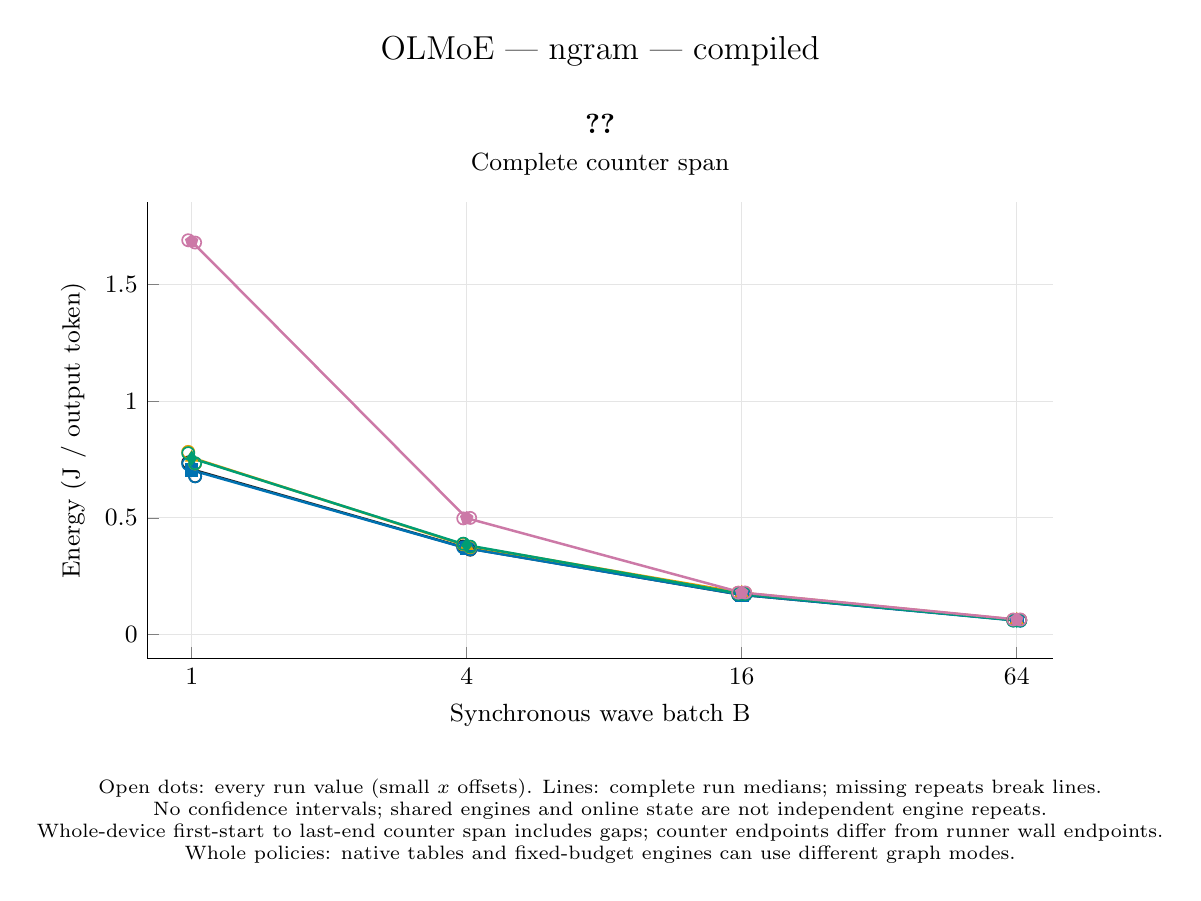
\begin{tikzpicture}
\definecolor{policy0}{HTML}{222222}
\definecolor{policy1}{HTML}{0072B2}
\definecolor{policy2}{HTML}{E69F00}
\definecolor{policy3}{HTML}{009E73}
\definecolor{policy4}{HTML}{CC79A7}
\begin{groupplot}[group style={group size=1 by 1,horizontal sep=2.0cm},width=11.5cm,height=5.8cm,scale only axis,grid=major,grid style={gray!20},axis lines*=left,unbounded coords=jump,xmode=log,log basis x=2,minor x tick num=0,scaled y ticks=false,tick label style={font=\small},label style={font=\small},title style={font=\small},xtick={1,4,16,64},xticklabels={1,4,16,64},xlabel={Synchronous wave batch B}]
\nextgroupplot[title={Complete counter span},ylabel={Energy (J / output token)},xmin=0.8,xmax=76.8,legend to name=policyLegend,legend columns=3,legend style={draw=none,font=\small,/tikz/every even column/.append style={column sep=8pt}}]
\addlegendimage{color=policy0,mark=*,line width=0.9pt}\addlegendentry{AR}
\addlegendimage{color=policy1,mark=square*,line width=0.9pt}\addlegendentry{Fixed gamma}
\addlegendimage{color=policy2,mark=triangle*,line width=0.9pt}\addlegendentry{Native table}
\addlegendimage{color=policy3,mark=diamond*,line width=0.9pt}\addlegendentry{Native threshold}
\addlegendimage{color=policy4,mark=pentagon*,line width=0.9pt}\addlegendentry{Adaptive}
\addplot[forget plot,color=policy0,mark=*,mark size=2pt,line width=0.9pt] coordinates {(1,0.708246520996) (4,0.37048223877) (16,0.169751281738) (64,0.0612135620117)};
\addplot[only marks,forget plot,color=policy0,mark=o,mark size=2.2pt,mark options={fill=white,line width=0.6pt}] coordinates {(0.982652235665,0.737671508789) (1.01765402215,0.678821533203) (3.93060894266,0.377424560547) (4.0706160886,0.363539916992) (15.7224357706,0.169679077148) (16.2824643544,0.169823486328) (62.8897430826,0.0610858154297) (65.1298574176,0.0613413085937)};
\addplot[forget plot,color=policy1,mark=square*,mark size=2pt,line width=0.9pt] coordinates {(1,0.704491333008) (4,0.369412109375) (16,0.17020513916) (64,0.0591992797852)};
\addplot[only marks,forget plot,color=policy1,mark=o,mark size=2.2pt,mark options={fill=white,line width=0.6pt}] coordinates {(0.982652235665,0.730984985352) (1.01765402215,0.677997680664) (3.93060894266,0.373558837891) (4.0706160886,0.365265380859) (15.7224357706,0.170613647461) (16.2824643544,0.169796630859) (62.8897430826,0.059958984375) (65.1298574176,0.0584395751953)};
\addplot[forget plot,color=policy2,mark=triangle*,mark size=2pt,line width=0.9pt] coordinates {(1,0.758264526367) (4,0.380455688477) (16,0.178693969727) (64,0.0627437744141)};
\addplot[only marks,forget plot,color=policy2,mark=o,mark size=2.2pt,mark options={fill=white,line width=0.6pt}] coordinates {(0.982652235665,0.783092041016) (1.01765402215,0.733437011719) (3.93060894266,0.386947875977) (4.0706160886,0.373963500977) (15.7224357706,0.17890625) (16.2824643544,0.178481689453) (62.8897430826,0.0627208251953) (65.1298574176,0.0627667236328)};
\addplot[forget plot,color=policy3,mark=diamond*,mark size=2pt,line width=0.9pt] coordinates {(1,0.755851257324) (4,0.383034484863) (16,0.173623168945) (64,0.0602006225586)};
\addplot[only marks,forget plot,color=policy3,mark=o,mark size=2.2pt,mark options={fill=white,line width=0.6pt}] coordinates {(0.982652235665,0.777614990234) (1.01765402215,0.734087524414) (3.93060894266,0.389367919922) (4.0706160886,0.376701049805) (15.7224357706,0.17386315918) (16.2824643544,0.173383178711) (62.8897430826,0.0595415039063) (65.1298574176,0.0608597412109)};
\addplot[forget plot,color=policy4,mark=pentagon*,mark size=2pt,line width=0.9pt] coordinates {(1,1.68596948242) (4,0.498867492676) (16,0.179612670898) (64,0.0641337280273)};
\addplot[only marks,forget plot,color=policy4,mark=o,mark size=2.2pt,mark options={fill=white,line width=0.6pt}] coordinates {(0.982652235665,1.69098010254) (1.01765402215,1.6809588623) (3.93060894266,0.497823608398) (4.0706160886,0.499911376953) (15.7224357706,0.179265991211) (16.2824643544,0.179959350586) (62.8897430826,0.0640764160156) (65.1298574176,0.0641910400391)};
\end{groupplot}
\path (group c1r1.north west) -- node[above=1.6cm,font=\large] {OLMoE | ngram | compiled} (group c1r1.north east);
\path (group c1r1.north west) -- node[above=0.75cm] {\ref{policyLegend}} (group c1r1.north east);
\path (group c1r1.south west) -- node[below=1.4cm,align=center,font=\scriptsize] {Open dots: every run value (small $x$ offsets). Lines: complete run medians; missing repeats break lines.\\No confidence intervals; shared engines and online state are not independent engine repeats.\\Whole-device first-start to last-end counter span includes gaps; counter endpoints differ from runner wall endpoints.\\Whole policies: native tables and fixed-budget engines can use different graph modes.} (group c1r1.south east);
\end{tikzpicture}\end{document}
